\documentclass[aps,twocolumn,showpacs]{revtex4-1}


\usepackage{epsfig}
\usepackage{amsfonts}
\usepackage{amssymb}
\usepackage{mathrsfs}
\usepackage{theorem}
\usepackage{amsmath}
\usepackage{times}
\usepackage{color}
\usepackage[french]{babel}
\usepackage[T1]{fontenc}
\usepackage{ifpdf}
\ifpdf
\usepackage{epstopdf}   
\usepackage{url}
\fi


\begin{document}
\title{Mechanical and relaxation-based detection of dipolar-interactions between spins in diamond}

\author{Clément Pellet-Mary$^1$, Maxime Perdriat$^1$, Paul Huillery$^1$, and Gabriel Hétet$^{1*}$}

\affiliation{$^1$Laboratoire de Physique de l’Ecole Normale Supérieure, ENS, Université PSL, CNRS, Sorbonne Université, Université de Paris, F-75005 Paris, France.\\$^*$ gabriel.hetet@phys.ens.fr
}

\begin{abstract}
\normalsize
The negatively charged nitrogen vacancy center (NV$^-$) is a well established quantum system, employed both for applications and fundamental research, thanks to its good coherence properties, long lifetimes and most importantly their ability to be optically polarized.
We have recently found new ways to use these properties of NV centers in order to study the dipolar interactions between ensemble of spins in diamond, including NV centers as well as other spin defects. 

On the one hand, we have observed cross-relaxations (CR) between NV centers and other defects (see Fig. 1), namely VH$^-$ \cite{VH}, War1 (first defect found by EPR at the university of Warwick, still chemically unknown) and $^{13}$C First-shell modified NV. None of these defects had been observed through CR before. This is a first step toward hyper-polarization of new spin defects in diamond.

On the other hand, we have used the mechanical detection of a levitating diamond \cite{nature} to measure the torque applied by the NV centers on the diamond when two classes of NV with different orientation are brought into resonance(see Fig. 2). This effect is due to the dipolar-mediated modification of the T$_1$ of NV centers happening with dense ensembles.\cite{Lukin}. This paves the way toward the mechanical detection of other spin impurities in diamond, as well as the observation of the Einstein-de Haas effect with paramagnetic systems. \cite{Meriles}

\begin{center}
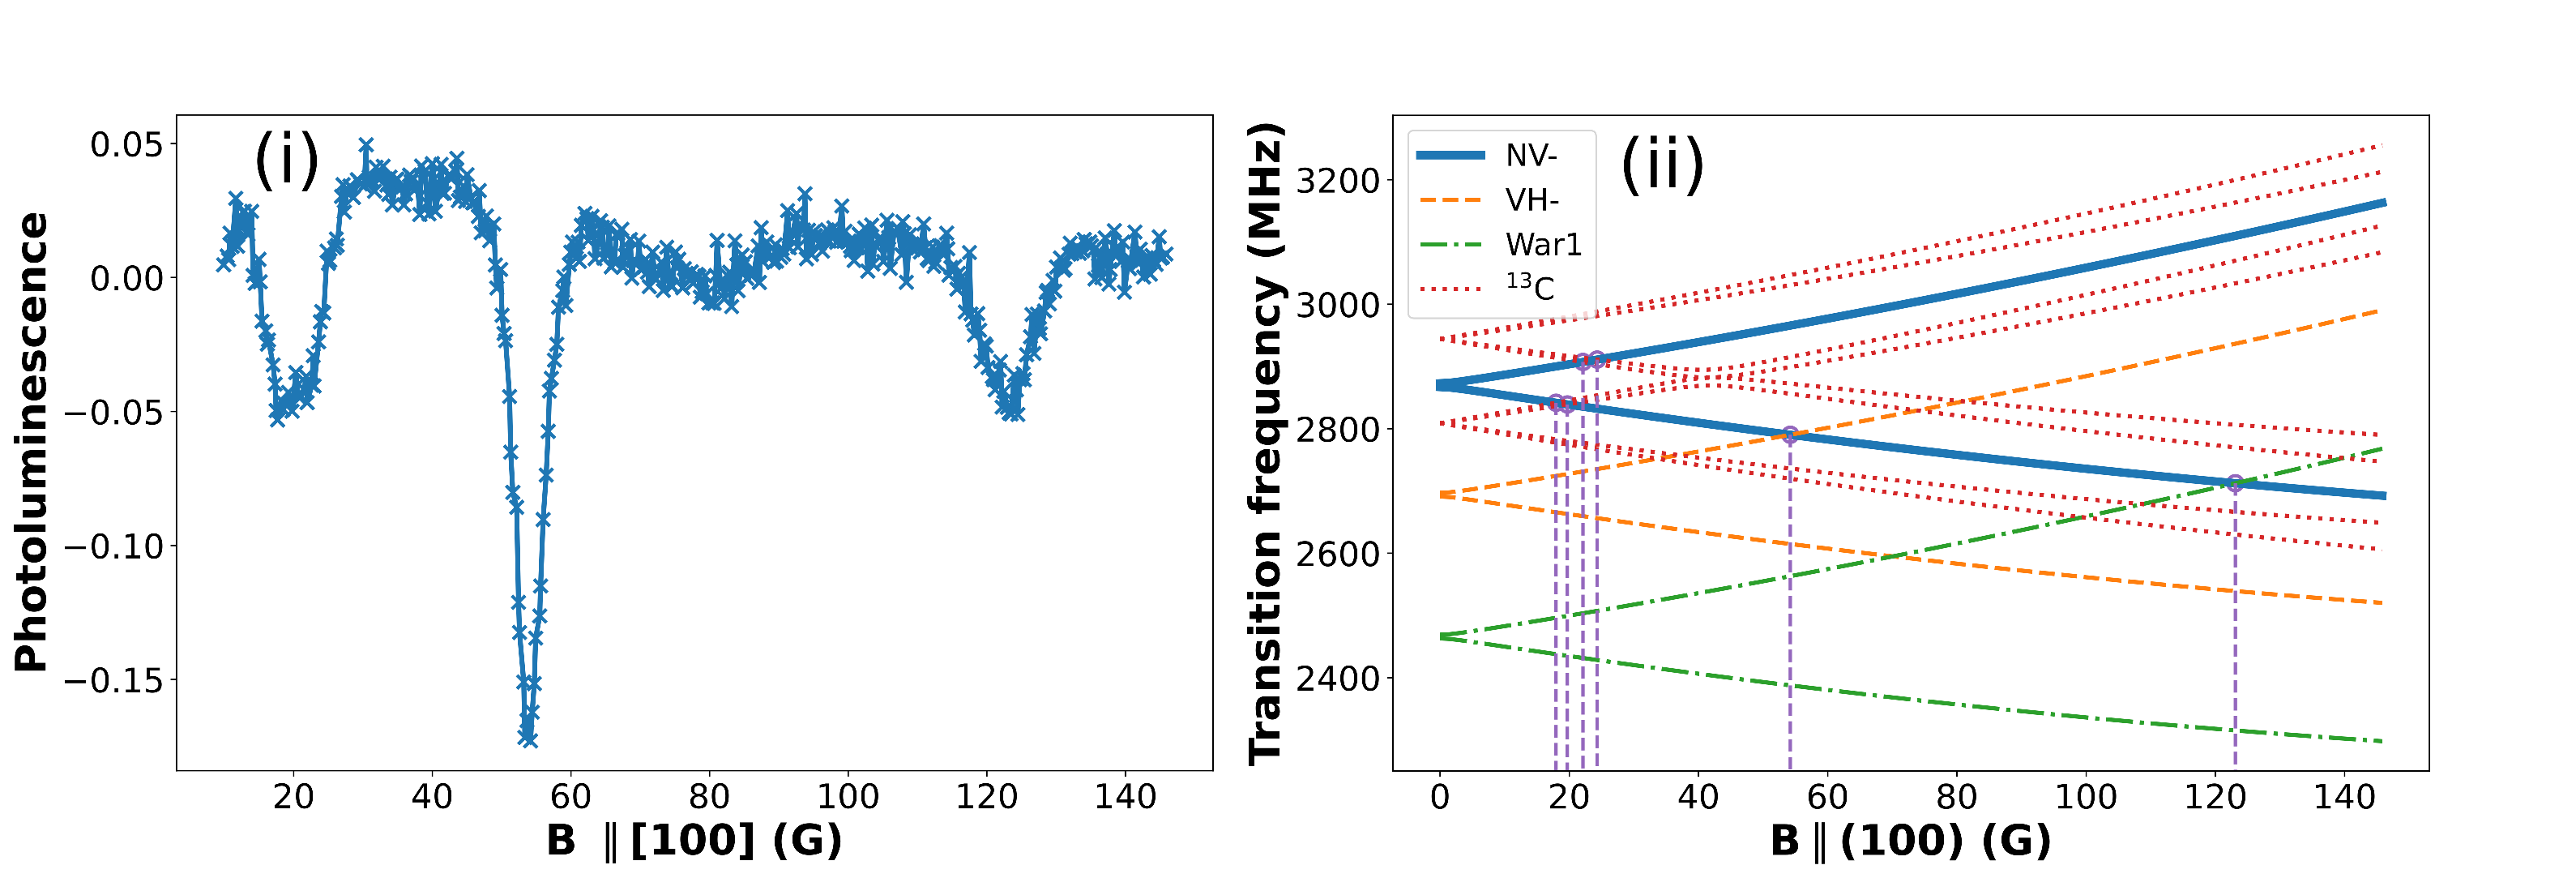
\includegraphics[scale=.25]{CR_total}
\end{center}

Figure 1 : Photoluminescence change while scanning the magnetic field along the crystalline [100] direction. Three dips are observed for the CR with $^{13}$C-NV, VH$^-$ and War1.

\begin{center}
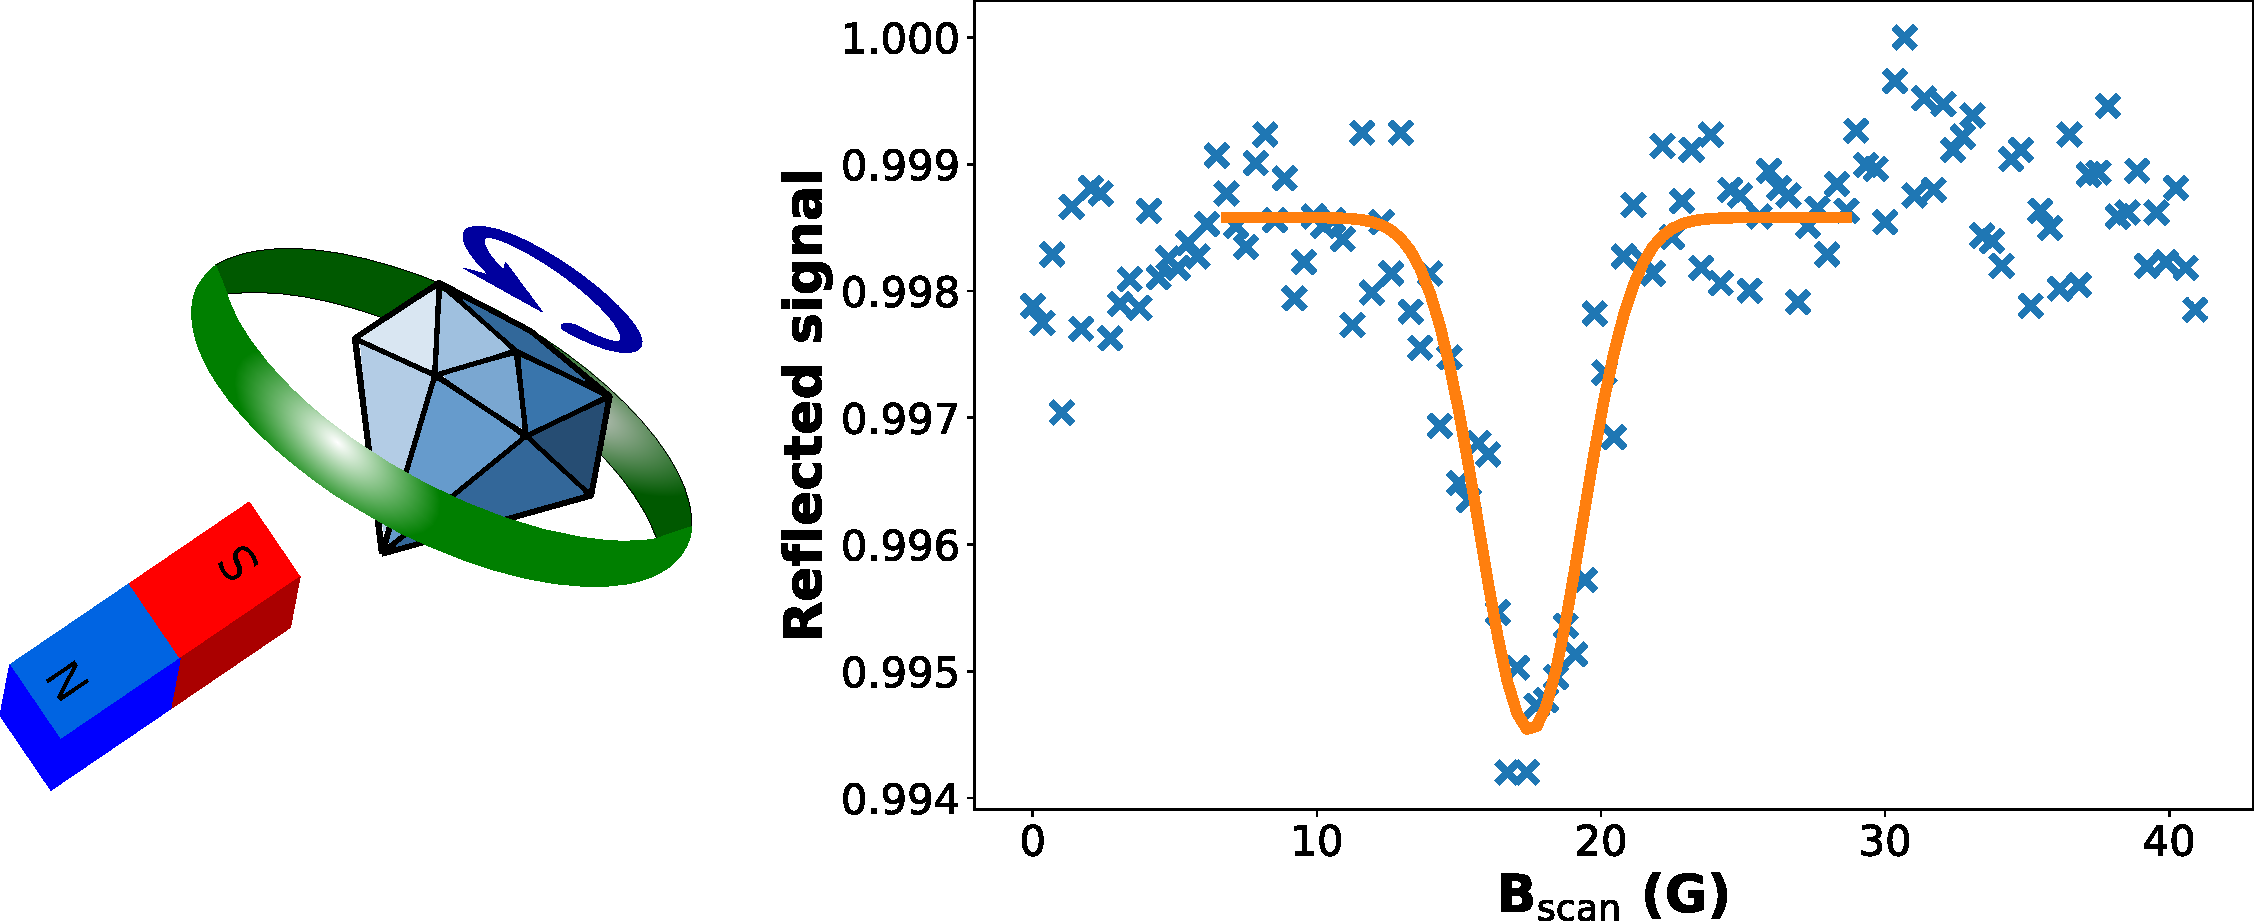
\includegraphics[scale=.25]{CRmeca_2}
\end{center}

Figure 2 : Angular position of the diamond while scanning B$_{\mathrm{Scan}}$ without a microwave. The rotation of the diamond at 17 G corresponds to the resonance between two classes of NV
\end{abstract}

\maketitle

\begin{thebibliography}{}

\bibitem{VH} Glover, C., et al. Physical review letters 90.18 (2003): 185507.

\bibitem{nature} Delord, T., et al. Nature 580.7801 (2020): 56-59.

\bibitem{Lukin} Choi, J., et al. Physical review letters 118.9 (2017): 093601.

\bibitem{Meriles} Zangara, P.R., et al. Physical Review B 100.23 (2019): 235410.

\end{thebibliography}
\end{document}
